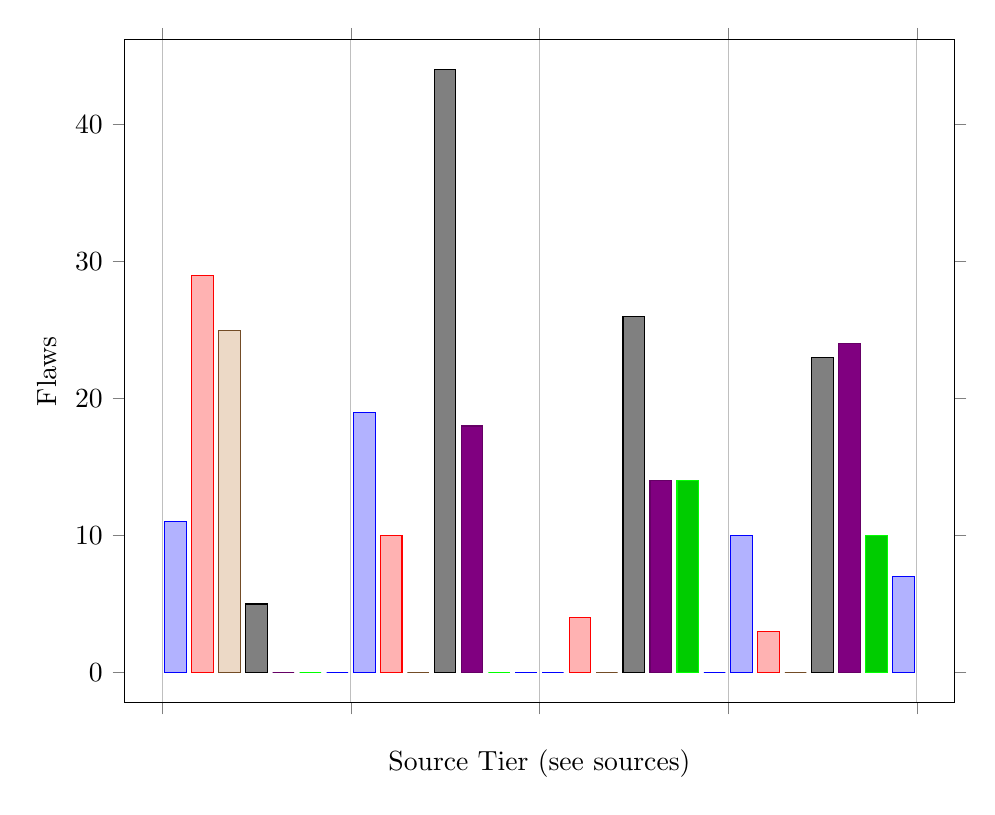
\begin{tikzpicture}
\begin{axis}[
width=\textwidth, height=10cm,
symbolic x coords={std,meta,text,paper,infer},
x tick label as interval,
xticklabels={{\parbox{0.16\textwidth}{\centering \stds{}}},{\parbox{0.16\textwidth}{\centering \metas{}}},{\parbox{0.16\textwidth}{\centering \texts{}}},{\parbox{0.16\textwidth}{\centering \papers{}}},{\parbox{0.16\textwidth}{\centering \infers{}}}},
xlabel=Source Tier (see \Cref{sources}), ylabel=Flaws,
enlargelimits=0.05, xbar=0pt, ybar interval=0.8,
]
\addplot coordinates {(std, 11) (meta, 19) (text, 0) (paper, 10) (infer, 0)};
\addplot coordinates {(std, 29) (meta, 10) (text, 4) (paper, 3) (infer, 0)};
\addplot coordinates {(std, 25) (meta, 0) (text, 0) (paper, 0) (infer, 0)};
\addplot coordinates {(std, 5) (meta, 44) (text, 26) (paper, 23) (infer, 0)};
\addplot coordinates {(std, 0) (meta, 18) (text, 14) (paper, 24) (infer, 0)};
\addplot coordinates {(std, 0) (meta, 0) (text, 14) (paper, 10) (infer, 0)};
\addplot coordinates {(std, 0) (meta, 0) (text, 0) (paper, 7) (infer, 0)};
\end{axis}
\end{tikzpicture}
